\documentclass[10pt]{book}

%These tell TeX which packages to use.
\usepackage{array,epsfig}
\usepackage{amsmath}
\usepackage{amsfonts}
\usepackage{amssymb}
\usepackage{amsxtra}
\usepackage{amsthm}
\usepackage{mathrsfs}
\usepackage{color}
\usepackage{enumitem}
%\usepackage{mdframed}
\usepackage[most]{tcolorbox}
\usepackage{pgfplots}
\pgfplotsset{compat=1.6}

\pgfplotsset{soldot/.style={color=black,only marks,mark=*}} \pgfplotsset{holdot/.style={color=black,fill=white,only marks,mark=*}}

%Here I define some theorem styles and shortcut commands for symbols I use often
\theoremstyle{definition}
\newtheorem{defn}{Definition}
\newtheorem{thm}{Theorem}
\newtheorem{cor}{Corollary}
\newtheorem*{rmk}{Remark}
\newtheorem{lem}{Lemma}
\newtheorem*{joke}{Joke}
\newtheorem{ex}{Example}
\newtheorem*{soln}{Solution}
\newtheorem{prop}{Proposition}

\newcommand{\lra}{\longrightarrow}
\newcommand{\ra}{\rightarrow}
\newcommand{\surj}{\twoheadrightarrow}
\newcommand{\graph}{\mathrm{graph}}
\newcommand{\bb}[1]{\mathbb{#1}}
\newcommand{\Z}{\bb{Z}}
\newcommand{\Q}{\bb{Q}}
\newcommand{\R}{\bb{R}}
\newcommand{\C}{\bb{C}}
\newcommand{\N}{\bb{N}}
\newcommand{\M}{\mathbf{M}}
\newcommand{\m}{\mathbf{m}}
\newcommand{\MM}{\mathscr{M}}
\newcommand{\HH}{\mathscr{H}}
\newcommand{\Om}{\Omega}
\newcommand{\Ho}{\in\HH(\Om)}
\newcommand{\bd}{\partial}
\newcommand{\del}{\partial}
\newcommand{\bardel}{\overline\partial}
\newcommand{\textdf}[1]{\textbf{\textsf{#1}}\index{#1}}
\newcommand{\img}{\mathrm{img}}
\newcommand{\ip}[2]{\left\langle{#1},{#2}\right\rangle}
\newcommand{\inter}[1]{\mathrm{int}{#1}}
\newcommand{\exter}[1]{\mathrm{ext}{#1}}
\newcommand{\cl}[1]{\mathrm{cl}{#1}}
\newcommand{\ds}{\displaystyle}
\newcommand{\vol}{\mathrm{vol}}
\newcommand{\cnt}{\mathrm{ct}}
\newcommand{\osc}{\mathrm{osc}}
\newcommand{\LL}{\mathbf{L}}
\newcommand{\UU}{\mathbf{U}}
\newcommand{\support}{\mathrm{support}}
\newcommand{\AND}{\;\wedge\;}
\newcommand{\OR}{\;\vee\;}
\newcommand{\Oset}{\varnothing}
\newcommand{\st}{\ni}
\newcommand{\wh}{\widehat}
%Pagination stuff.
\setlength{\topmargin}{-0.75in}
\setlength{\oddsidemargin}{0in}
\setlength{\evensidemargin}{0in}
\setlength{\textheight}{9.in}
\setlength{\textwidth}{6.5in}
\pagestyle{empty}
\begin{document}
\begin{flushleft}
Name:\underline{\hspace{13cm}}Date:\underline{\hspace{2cm}}
\end{flushleft}
\begin{center}
{\Large Math 1041-012 \hspace{0.5cm} Section 2.6: Limits at Infinity}
\end{center}
%\vspace{0.2 cm}
\subsection*{Intro. Example} Consider the function $\displaystyle f(x)=\frac{x^2-1}{x^2+1}$ and below is its graph:
\begin{figure}[h!]
\centering
    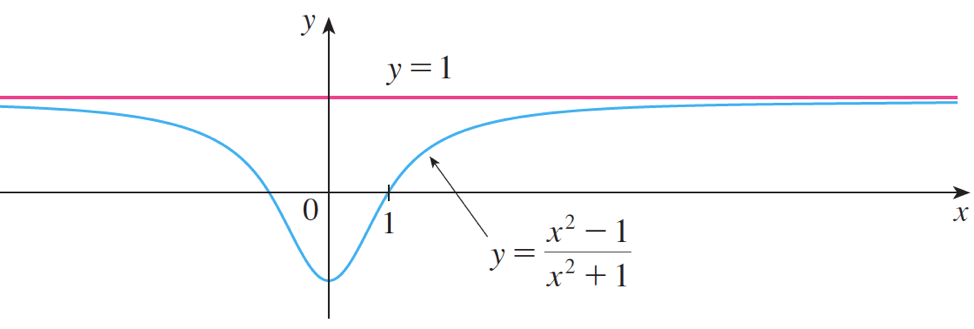
\includegraphics[scale=0.75]{fig1.png}
\end{figure}
\begin{itemize}
    \item[(a)] How do we describe the \textit{long term} behavior of $f(x)$?\vspace{1cm}
    \item[(b)] How do we describe long term behavior using limits?
\end{itemize}
\vspace{1cm}
\begin{tcolorbox}
\subsection*{Definition} Let $f(x)$ be defined on a large interval:
\begin{itemize}
    \item[(a)] For $f$ defined on $(a,\infty)$ then
    \[
    \lim_{x\rightarrow \infty}f(x)=L
    \]
    is a limit at $\infty$, which means:
    \vspace{0.5cm}
    \item[(b)] For $f$ defined on $(-\infty,a)$ then
    \[
    \lim_{x\rightarrow -\infty}f(x)=L
    \]
    is a limit at $-\infty$, which means:\vspace{0.5cm}
\end{itemize}
\end{tcolorbox}
There are many ways that a function can behavior in the long term:
\begin{figure}[h!]
    \centering
    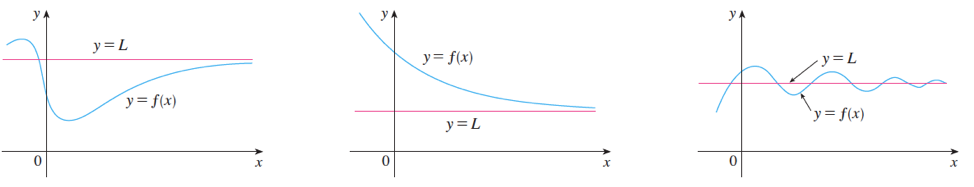
\includegraphics[scale=0.75]{fig2.png}
\end{figure}
\raggedbottom
\clearpage
\begin{tcolorbox}
\subsection*{Definition Horizontal Asymptotes}
The line $y=L$ is called a \textbf{horizonal asymptote} of the curve $y=f(x)$ if either
\[
\lim_{x\rightarrow -\infty}f(x)=L\ \text{ or } \lim_{x\rightarrow \infty}f(x)=L
\]
\end{tcolorbox}
\subsection*{Example 1: ArcTan}
Find the horizontal asymptotes of $y=\tan^{-1}x$. Make a sketch!\vspace{4cm}
\subsection*{Example 2: Limits from a Graph}
Identity the asymptotes in the graph below AND write the corresponding limtis!
\begin{figure}[h!]
    \centering
    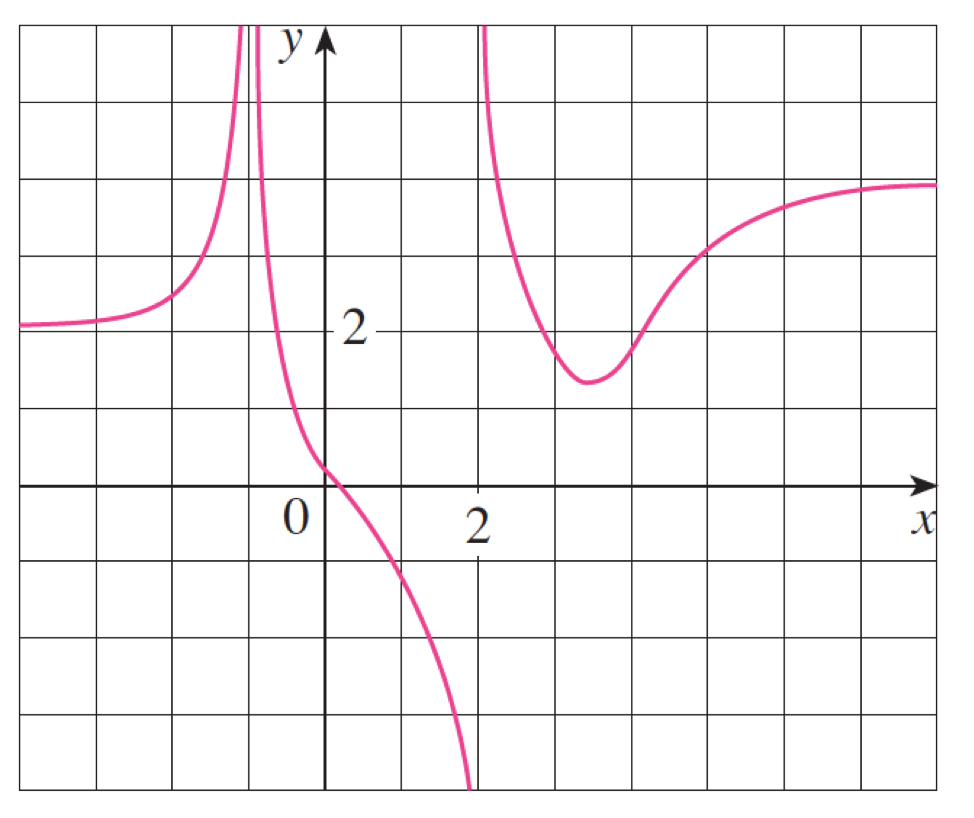
\includegraphics[scale=0.55]{fig3.png}
\end{figure}
\clearpage
\subsection*{Example 3: Find and Sketch a function}
Sketch a function such that
\[
\lim_{x\rightarrow -\infty}f(x)=0\ \ \text{ and } \lim_{x\rightarrow \infty}f(x)=0.
\]
Think of a function that behaves like this!\vspace{2cm}
\begin{tcolorbox}
\subsection*{Theorem}
If $r>0$ is a rational number then
\[
\lim_{x\rightarrow \infty}\frac{1}{x^r}=0
\]
If $r>0$ is a rational number such that $x^r$ is defined for every $x$ (why??) then
\[
\lim_{x\rightarrow -\infty}\frac{1}{x^r}=0
\]
\end{tcolorbox}
\subsection*{Example 4: Using the Theorem}
\begin{itemize}
    \item[(a)] Evaluate $\displaystyle\lim_{x\rightarrow \infty}\frac{3x^2-x-2}{5x^2+4x+1}$ and  $\displaystyle\lim_{x\rightarrow -\infty}\frac{3x^2-x-2}{5x^2+4x+1}$\vspace{6cm}
    \item[(b)] Find the horizontal and vertical asymptotes of $\displaystyle f(x)=\frac{\sqrt{2x^2+1}}{3x-5}$
\end{itemize}
\raggedbottom
\clearpage
\subsection*{Example 5: Tricky Limit}
\begin{itemize}
\item[(a)] Compute $\displaystyle\lim_{x\rightarrow \infty}\sqrt{x^2+1}-x$.\\
\vspace{3cm}
\item[(b)] Compute $\displaystyle \lim_{x\rightarrow 2^+}\arctan\left(\frac{1}{x-2}\right)$
\vspace{3cm}
\end{itemize}
\begin{tcolorbox}
\subsection*{Rule for Exponential}
\[\lim_{x\rightarrow -\infty}e^x=0\]

Why?
\end{tcolorbox}
\subsection*{Some Tricky Examples}
\begin{itemize}
    \item[(a)] Compute $\displaystyle \lim_{x\rightarrow 0^-}e^{1/x}$\vspace{4cm}
    \item[(b)] Compute $\displaystyle\lim_{x\rightarrow \infty}\sin x$.
\end{itemize}
\raggedbottom
\clearpage
\begin{tcolorbox}
\subsection*{Infinite Limits at Infinity}
The notation
\[
\lim_{x\rightarrow \infty}f(x)=\infty
\]
reads as: \\ \\
This indicates that as $x$ becomes arbitrarily large then $f(x)$ becomes large. Similar meanings for
\[
\lim_{x\rightarrow -\infty}f(x)=\infty,\ \ \ \lim_{x\rightarrow \infty}f(x)=-\infty,\ \ \ \lim_{x\rightarrow -\infty}f(x)=-\infty
\]
\end{tcolorbox}
\subsection*{Some Examples}
\begin{itemize}
    \item[(a)] Find $\displaystyle\lim_{x\rightarrow \infty}e^x$\vspace{4cm}
    \item[(b)]Find $\displaystyle\lim_{x\rightarrow \infty}x^2-x$\vspace{4cm}
    \item[(c)]Find
    $\displaystyle\lim_{x\rightarrow \infty}\frac{x^2+x}{3-x}$
\end{itemize}
\raggedbottom
\clearpage
\subsection*{Example: Sketching}
Sketch the graph of $y=(x-2)^4(x+1)^3(x-1)$ by finding its intercepts and its limits as $x\rightarrow -\infty$ and $x\rightarrow \infty$.
\end{document}